\only<beamer>{\titleframe}




\begin{frame}{Overview}
    \tableofcontents
\end{frame}




\sectionframe{General facts about Fellbach}

\section{General facts}

\begin{frame}{General facts}
    Population about 46.000\\
    Size 27.71 $km^2$\\
    First citation 1121 A.D.\\
    Split up into 3 regions (Fellbach, Schmiden, Oeffingen)


\end{frame}

\begin{frame}{Map}


    \begin{figure}
        \centering
        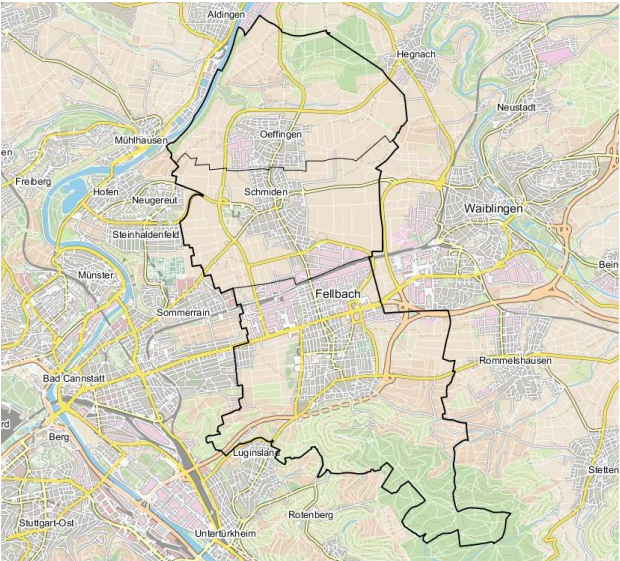
\includegraphics[width=175pt]{gfx/logos/fellbachMap}
        \caption{Map of Fellbach}
        \label{fig:Fellbach}
    \end{figure}
\end{frame}



\sectionframe{The Three Districs in Comparison}

\section{Comparison}

\begin{frame}{Comparison}
    \begin{table}[!h]
        \centering
        \begin{tabular} {| c | c | c |}
            \hline Name of District & Population & Size\\
            \hline Fellbach & about 23200 & 15,54 $km^2$\\
            \hline Schmiden &  about 15900 & 7,21 $km^2$\\
            \hline Oeffingen & about 6900 & 4,96 $km^2$
        \end{tabular}
        \caption{The Three Districts of Fellbach in Comparison}
        \label{tab:Comparison}
    \end{table}
\end{frame}

\sectionframe{Sightseeing in Fellbach}

\section{Sightseeing}

\begin{frame}{Worthwile Sights}
    \begin{enumerate}
        \item Kappelberg
        \pause \item Alte/Neue Kelter
        \pause \item Max-Graser-Stadion and the Adventure Playground
        \pause \item Schwabenlandhalle
    \end{enumerate}

\end{frame}



\thanksframe
